\documentclass[11pt, openany]{book}              % Book class in 11 points
\parindent0pt  \parskip10pt             % make block paragraphs
\raggedright                            % do not right justify
\usepackage{graphicx}
%\graphicspath{ {./images/} }
\title{\bf Quantitative Investment Handbook}    % Supply information
\author{Xinhe Liu}              %   for the title page.
\date{2018-2-28}                           %   Use current date. 

% Note that book class by default is formatted to be printed back-to-back.
\begin{document}                        % End of preamble, start of text.
% \frontmatter                            % only in book class (roman page #s)
\maketitle                              % Print title page.
\tableofcontents                        % Print table of contents
\mainmatter                             % only in book class (arabic page #s)


\chapter{Basic Financial Concepts}                % Print a "chapter" heading

This chapter summarizes some basic financial concepts you should know about.
\section{Corporate Finance and Fundamental Analysis}

\begin{enumerate}
 \item NPV and IRR 
 \item Discounted Cash Flow Model
  \begin{itemize}
    \item Free Cashflow
    \item Required Rate of Return = Cost of Capital = Risk-adjusted discount rate : Usually from the CAPM
   \end{itemize}
 \item Valuation using Multiples - P/E, P/B 
 \end{enumerate}


\section{Asset Management}

\begin{enumerate}
 \item Efficient Market Hypothesis (Weak, Semi-strong, Strong forms)
 \item Markowitz Portfolio Optimization
 \begin{itemize}
    \item Minimum Variance Portfolio / Tangency Portfolio 
    \item Jensen's alpha
  \end{itemize}

  \item Capital Asset Pricing Model(CAPM) Model \\
        $$ r = \beta(r_m - r_f) + r_f $$
 		$$\beta = \frac{cov(r,r_M)}{var(r_M)}$$
  \item APT(Arbitrage-Free-Pricing) Model 
 \item No-arbitrage(weak, strong) and Law-of-one-price
 \item Metrics
  \begin{itemize}
    \item Sharpe Ratio
    \item Jensen's alpha
    
        \item Required Rate of Return = Cost of Capital = Risk-adjusted discount rate : Usually from the CAPM
   \end{itemize}
 \item Valuation using Multiples - P/E, P/B 
 \end{enumerate}


\chapter{Portfolio Optimization Study}

  One-fund theorem, two fund theorem 


   convex reformulation of maximizing Sharpe ratio problem(normalizing) 


  Multi-factor Risk Model 
    r = Bf + u ~ V = Bcov(f)B^T + cov(u) 

   
   Mixed Integer Optimization


   Stochastic and Dynamic Optmization


Issue 


	Active Holding Optimization
              optimize alpha holdings and tracking error



Improvements on MVO
   estimation error
  	Shrinkage estimators
		Jason-Stein Estimator  
	Black-Litterman Model
	Robust Estimators

    optimization issue
	add constraints
	resampled efficiency
	use other diversification approach 
		risk-parity 
  		maximize diversification		




Mixed Integer Optimization

Heuristic
  forward
  backward selection
  clustering


Stochastic Optimization
scenario optmization approach
Var
cVar

 Kelly’s Crirterion 

Multi-period optmization room




Excel solver
 CVX matlab
CVXOPT python
optmization toolbox matlab
Gorubi




\section{Estimating Return and Co-variance Matrix}
\section{Transaction Cost}
\section{Tax}
\section{Dynamic Portfolio Choice}
\section{Covariance Matrix}

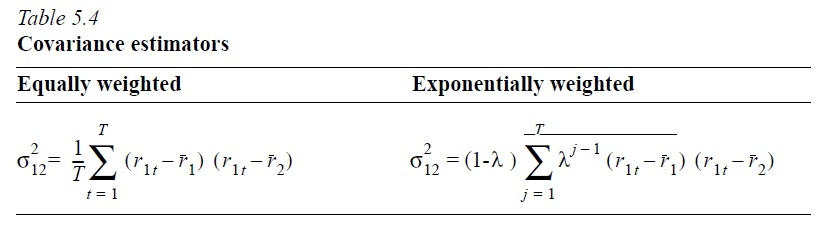
\includegraphics[scale=0.5]{Cov.JPG}

\section{Easy}
\begin{enumerate}
 \item Two coins, one is double tail, you see one \\
  \begin{itemize}
    \item three pancakes: golden-golden, golden-brunt, brunt-brunt, see one golden, probability that the other side is golden two
    \item 
   \end{itemize}
 \item Two coins - one toss n+1, one toss n, probability that n+1 gets more tail than n man?
\end{enumerate}


\section{Medium}
\begin{enumerate}
	\item Use coins to create probabilities : fair coin to create 1/3 probability - toss twice, one result is retoss
unfair coin to create 1/3 probability - combine two toss as one


 \end{enumerate}
 
\section{Hard}
\chapter{Statistical Arbitrage}

\section{mean-reversion}

intraday mean-reversion


\chapter{Volatility Trading and Dispersion Trading}

\section{Volatility Models and Time-Series Models}

Volatility Clustering and Leverage Effect 

\chapter{Index and Smart Beta}
 
\section{Smart beta and Smart Alpha}                  % Print a "section" heading
\section{Key things to Notice in Index Making}
\section{factor analysis and risk premia}

value, momementum, quality, volatility, betaRM-RF  The return spread between the capitalization weighted stock market and cash.

QUality Minus Junk (quanlity)

SMB      The return spread of small minus large stocks (i.e., the size effect).

HML      The return spread of cheap minus expensive stocks (i.e., the value effect).

RMW     The return spread of the most profitable firms minus the least profitable.

CMA      The return spread of firms that invest conservatively minus aggressively.

UMD (momentum/trend) UMD is long winners and short losers and also from Ken French’s website)

Carry  Vol Carry


Special: liquidity premia 


Market Ineffciency Analysis: funding constraint of financial institutions, grand move of large funds constraints

\section{Market Anomalies}

Behavioral Market Anomalies/bias


other: liquidity risk premia
\begin{enumerate}
 \item Risk Management and Hedging 
 \item Leverage 
 \item Correlation
 \item Strategy replacements, leverage rebalancing and rebalancing frequency, leverage reset
\end{enumerate}



The following sectioning commands are available:
\begin{quote}                           % The following text will be
 part \\                                %    set off and indented.
 chapter \\                             % \\ forces a new line
 section \\ 
 subsection \\ 
 subsubsection \\ 
 paragraph \\ 
 subparagraph 
\end{quote}                             % End of indented text
But note that---unlike the \texttt{book} and \texttt{report} classes---the
\texttt{article} class does not have a ``chapter" command.

\chapter{Strategies Implementation/Platform Building}
\section{ Trading System }
\section{ Strategy Development Pipeline(Single/Linear Strategy) }
\subsection{Basic Architecture/System}
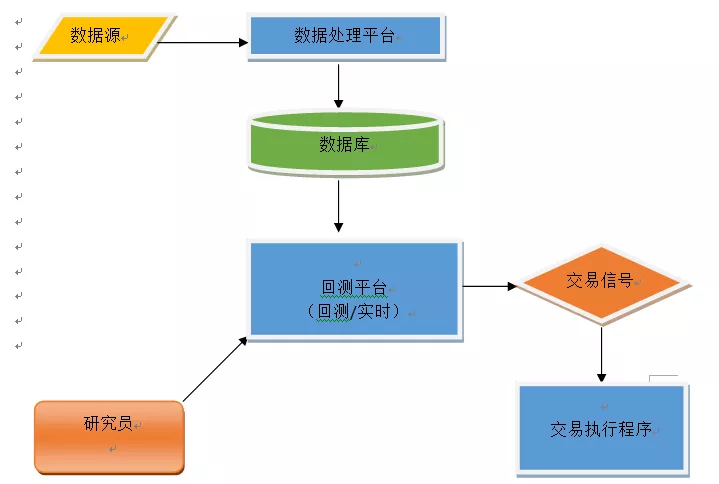
\includegraphics[scale=0.5]{1.JPG}
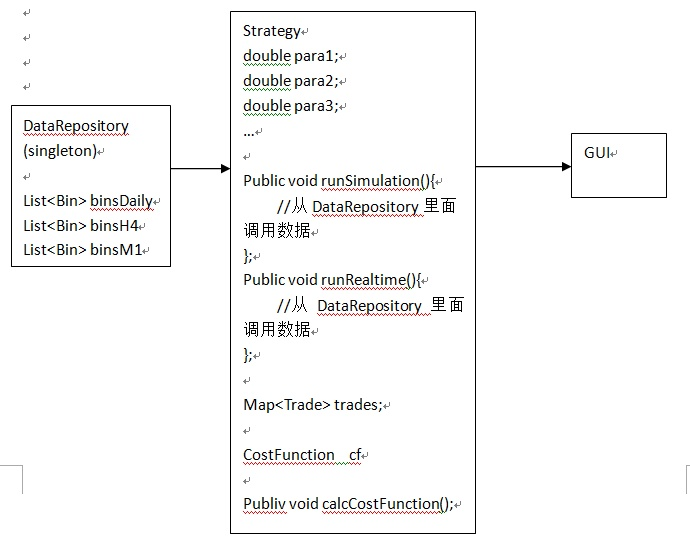
\includegraphics[scale=0.5]{2.JPG}
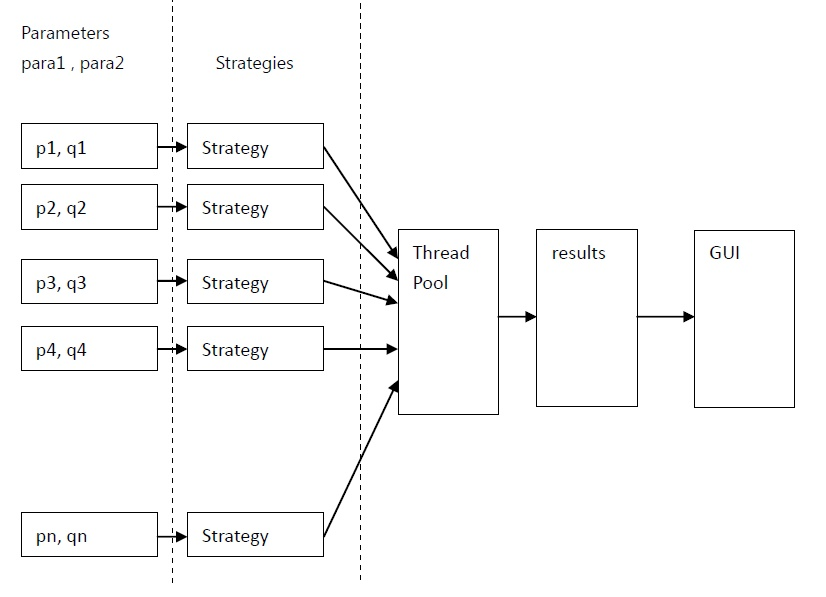
\includegraphics[scale=0.5]{3.JPG}
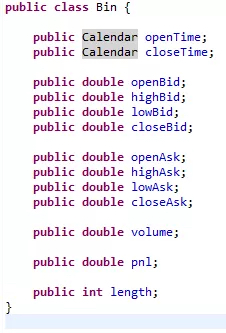
\includegraphics[scale=0.5]{4.JPG}
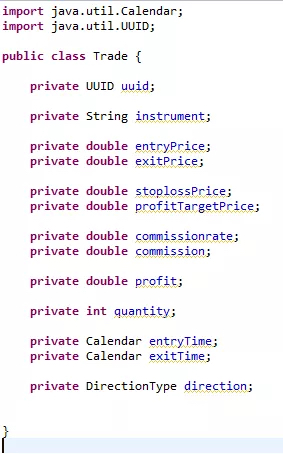
\includegraphics[scale=0.5]{5.JPG}
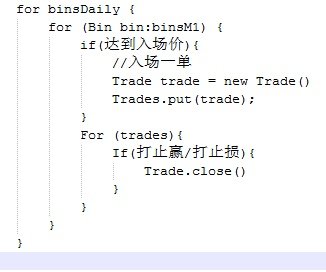
\includegraphics[scale=0.5]{6.JPG}


Historical Data is a singleton. All Market Data (eg. a candle stick ) should be organized to feed the researcher to program strategies on the backtester (eg. like quantopian). All back-testing should be parallized (ideally on GPU) to display parameter-profit relationship. (heatmap, stock charts, etc ) Ideally the optimization process could be visualized (like Tensorflow) 

All like a research facility feedback cycle. 

Key Details: API Design, Module Separation etc. 
\subsection{Data}

Key is a real-time listener. Technical Considerations: KDB, Hadoop and HDFI(?), SQL Like, Mongo Db to store Archive Data. Market Data Providers consideration buying from Wind, BBG, Reuters, Etc. \\

teams: platform operation engineer, analytics builder, strategy control/management and risk management, data team, execution team, researcher team ( 3 x tech )\\

data licensing and data quality insurance \\

data base, text file archive, big data issue\\

cheap data: brokerage: interative brokers.

\subsection{Backtester/Simulator}

Key Components

*Send Singal to Quoting/Trading/Exection Tool(Real Time)
*Market Data Objects (eg. loop for every time bins)
*stop loss/risk control system integration
*parameter-backtest profit/statistics result: optimization and loss function set function to tune the parameters
*multi-thread: Java backter (Java thread pool*)
*human selection of parameters: parameter table and visualization

\subsection{Trade Record and Money Management}

record every trade, summarize execution shortfall, statistical trends and information (shortcomings of strategy executions) and market information ( learning material) build statistics and storage

More: order book and trade book level data handling

\subsection{Analytics}

\subsubsection{ Strategy Management }, Sharpe Anslysis, Holding Period, Slippage visualization to better assistant strategic allocation

\subsubsection{Execution Analysis and Cost}

quantitative trading/systematic trading strategies:
* equity long/short

\subsection{Research Team}
Key problems:
* Optimization and Combination of Sub-Strategies (Eg. factors)
* Market Regime Change Detection(problem not solved): Distinguish between trend and oscillation market
* market supply/demand imbalance analysis (risk-premia) 
* volatility trading, dispersion trading - 2nd and 3rd degree trading, (vol model, vol clustering effect, vol leverage effect)
* hedging/overlay strategy research: hedging cost and hedging risk management, how to adjust hedge according to market condition.
* common ideas: market imbalance, mean-reversion, autocorrelation patterns etc (find patterns and trade) - based on statistics.  Risk factors, implied arbitrage - based on math. 

\subsubsection{Parameter Optmization and Control}

Rely on GUI - parameter distribution and selection
optmization methdologies from machine learning ( see optimization chapter)
robustness anslysis and out-of sample test ** ( random cut the universe of rolling window on selection period )

\subsubsection{Signal Indicator Design}

For example, based on fundemental ratio and technical indicators - design a formula. And check the level of prediction power (if any)

1.seeking stationarity: find a stationary time series
	use difference, integration, and normalize with volatility 
2.find signal level, plot cumulative back-test return against different signal level (use own quotes, and use signal level to filter quotes)
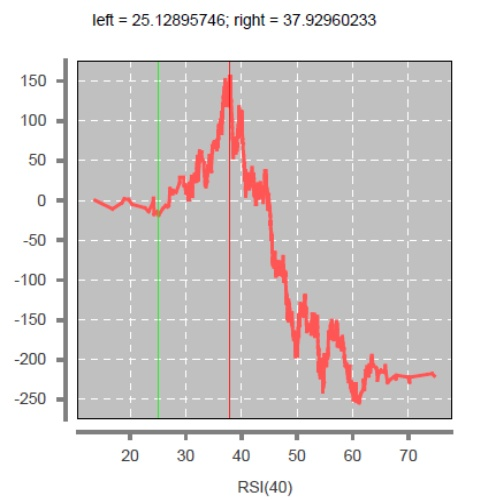
\includegraphics[scale=0.5]{7.JPG}
3.Check stability of customized indicators 
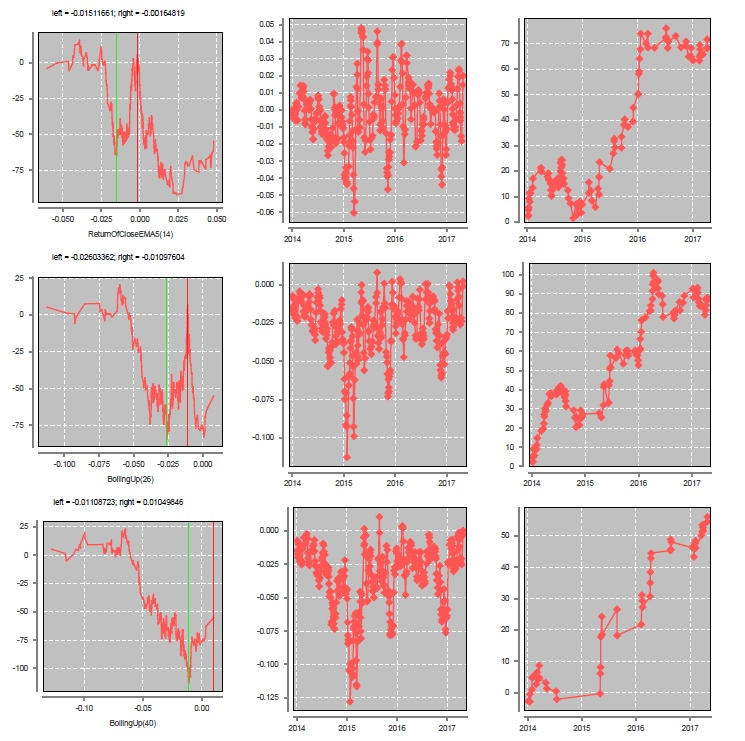
\includegraphics[scale=0.5]{8.JPG}
4. check overfitting and type-II error in all settings, apply noise filtering if possible 
5. design a interface to input indicator(math formula parser to read string) and visualize information using GUI.(HTML/XML Render)
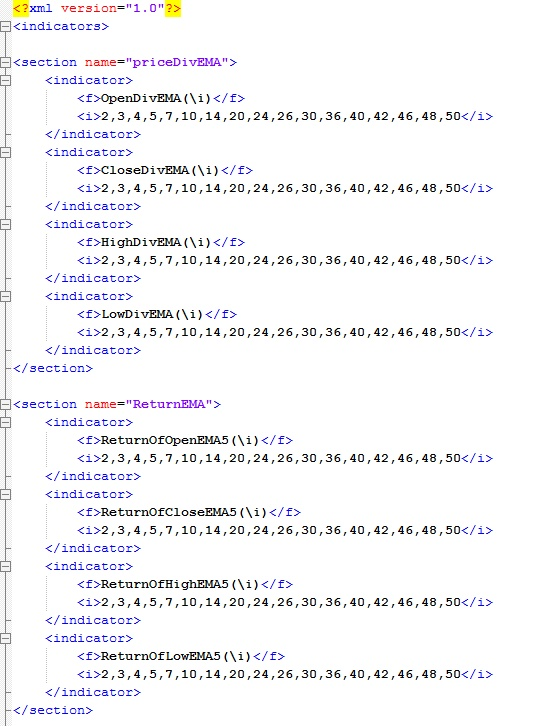
\includegraphics[scale=0.5]{9.JPG}
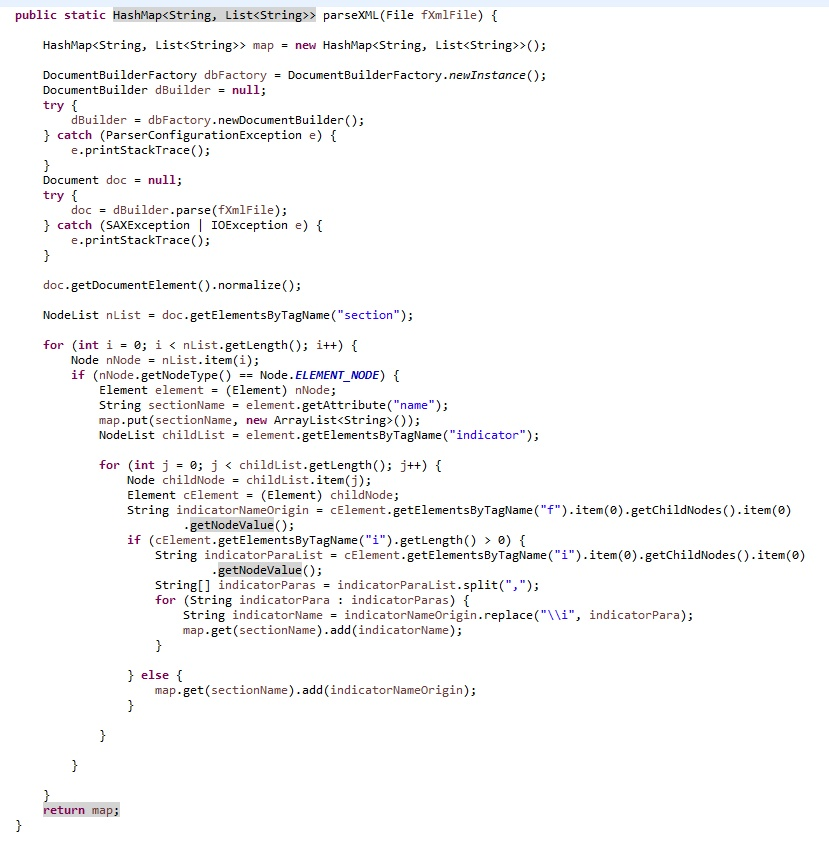
\includegraphics[scale=0.5]{10.JPG}
6. aggregate all indicators( eg. macd, ead ). Aggregate all strategies using optimization framework or selection framework to gain statistical alpha
7. indicator effectiveness test
1. test correlation - the correlation between indicator and profit vs. the correlation between correlation and white noise(hypothesis test) * use spearman correlation rather than pearson correlation* 
2. Use Monte Carlo Simulation to do permutation test of effectiveness of indicator
3. Very very hard - detect sensentivity to market regime change(osicallation and trend) and identify market regime change. 

\subssubsection{Integration of single indicators and portfolio theory}

Form indicator as factors: standardization to mean-0, normal/t-distributed scores. Select powerful ones (ones that passed the permutation test). Optimize to maximize holdings exposure to factor with risk penalty. The key is still feature engineering.

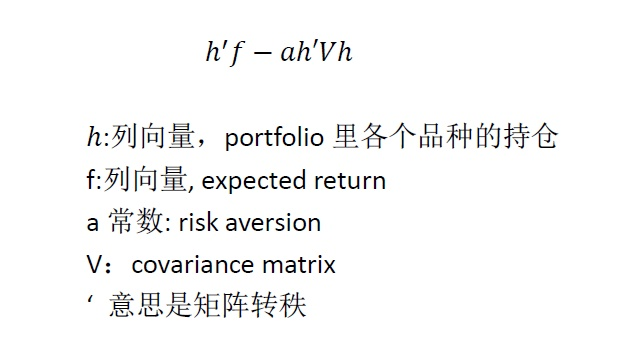
\includegraphics[scale=0.5]{11.JPG}

For Covariance, See section "covariance matrix".  



\subsubsection{Strategy Risk Management and Money management}

small stop loss, big stop gain level on reversion strategies.bigger stop loss, smaller stop gains on volatile markets - based on experience, market analysis.

Choose symmeteric/non-symmetric risk control based on market belief

Hedging and Market Exposture Management - Volatility Control and Automatic de-leveraging. 

together with cost consdieration. 


\chapter{Alternative Data}
 
\end{document}                          % The required last line 